% This is "sig-alternate.tex" V2.0 May 2012
% This file should be compiled with V2.5 of "sig-alternate.cls" May 2012
%
% This example file demonstrates the use of the 'sig-alternate.cls'
% V2.5 LaTeX2e document class file. It is for those submitting
% articles to ACM Conference Proceedings WHO DO NOT WISH TO
% STRICTLY ADHERE TO THE SIGS (PUBS-BOARD-ENDORSED) STYLE.
% The 'sig-alternate.cls' file will produce a similar-looking,
% albeit, 'tighter' paper resulting in, invariably, fewer pages.
%
% ----------------------------------------------------------------------------------------------------------------
% This .tex file (and associated .cls V2.5) produces:
%       1) The Permission Statement
%       2) The Conference (location) Info information
%       3) The Copyright Line with ACM data
%       4) NO page numbers
%
% as against the acm_proc_article-sp.cls file which
% DOES NOT produce 1) thru' 3) above.
%
% Using 'sig-alternate.cls' you have control, however, from within
% the source .tex file, over both the CopyrightYear
% (defaulted to 200X) and the ACM Copyright Data
% (defaulted to X-XXXXX-XX-X/XX/XX).
% e.g.
% \CopyrightYear{2007} will cause 2007 to appear in the copyright line.
% \crdata{0-12345-67-8/90/12} will cause 0-12345-67-8/90/12 to appear in the copyright line.
%
% ---------------------------------------------------------------------------------------------------------------
% This .tex source is an example which *does* use
% the .bib file (from which the .bbl file % is produced).
% REMEMBER HOWEVER: After having produced the .bbl file,
% and prior to final submission, you *NEED* to 'insert'
% your .bbl file into your source .tex file so as to provide
% ONE 'self-contained' source file.
%
% ================= IF YOU HAVE QUESTIONS =======================
% Questions regarding the SIGS styles, SIGS policies and
% procedures, Conferences etc. should be sent to
% Adrienne Griscti (griscti@acm.org)
%
% Technical questions _only_ to
% Gerald Murray (murray@hq.acm.org)
% ===============================================================
%
% For tracking purposes - this is V2.0 - May 2012

%\documentclass{sig-alternate}
\documentclass{sig-alternate}

\usepackage{makeidx}  % allows for indexgeneration
\usepackage{comment}



%% \usepackage[style=alphabetic]{biblatex}
% \usepackage[authoryear,sectionbib]{natbib}
%% \PassOptionsToPackage{authoryear}{natbib}
%% \usepackage{caption}
\usepackage{graphicx}
\usepackage{subfigure}
\usepackage{url}

\usepackage{paralist}
\usepackage{verbatim}
\usepackage{array}
\usepackage{float}
\usepackage{multirow}
% \usepackage{rotating}
\usepackage{multicol}
\usepackage{longtable}

\usepackage{listings} 	
% "define" Scala
\lstdefinelanguage{scala}{
  morekeywords={abstract,case,catch,class,def,%
    do,else,extends,false,final,finally,%
    for,if,implicit,import,match,mixin,%
    new,null,object,override,package,%
    private,protected,requires,return,sealed,%
    super,this,throw,trait,true,try,%
    type,val,var,while,with,yield},
  otherkeywords={=>,<-,<\%,<:,>:,\#,@, <:<},
  sensitive=true,
  morecomment=[l]{//},
  morecomment=[n]{/*}{*/},
  morestring=[b]",
  morestring=[b]',
  morestring=[b]"""
}


\usepackage{pxfonts}
\usepackage{color}
\definecolor{dkgreen}{rgb}{0,0.6,0}
\definecolor{gray}{rgb}{0.5,0.5,0.5}
\definecolor{mauve}{rgb}{0.58,0,0.82}
 
% Default settings for code listings
\lstset{frame=tb,
  language=scala,
  aboveskip=3mm,
  belowskip=3mm,
  showstringspaces=false,
  columns=flexible,
  basicstyle={\small\ttfamily},
  numbers=left, % none,
  numbersep=2pt,
  numberstyle=\tiny\color{gray},
  keywordstyle=\bfseries\color{black},
  commentstyle=\color{dkgreen},
  stringstyle=\color{black},
  frame=none, % single,
  breaklines=true,
  breakatwhitespace=true,
  tabsize=2,
  captionpos=b
}

\usepackage[pdfpagelabels]{hyperref}
\usepackage[all]{hypcap}


% A comment in a draft (shouldn't appear in the final version).
\newcommand{\mycomment}[1]{\(\spadesuit\){\bf #1 }\(\spadesuit\)}
% Comment this out in the draft
% \newcommand{\mycomment}[1]{}
\newcommand{\pmcomment}[1]{\comment{PM}{#1}}
\newcommand{\pwtcomment}[1]{\comment{PT}{#1}}
\newcommand{\rscomment}[1]{\comment{RS}{#1}}

% line break in table.  e.g.
% Foo bar & \specialcell{Foo\\bar} & Foo bar \\    % vertically centered
% Foo bar & \specialcell[t]{Foo\\bar} & Foo bar \\ % aligned with top rule
\newcommand{\specialcell}[2][c]{%
  \begin{tabular}[#1]{@{}c@{}}#2\end{tabular}}

 
\begin{document}
%
% --- Author Metadata here ---
\permission{Permission to make digital or hard copies of all or part of this work for personal or classroom use is granted without fee provided that copies are not made or distributed for profit or commercial advantage and that copies bear this notice and the full citation on the first page. Copyrights for components of this work owned by others than the author(s) must be honored. Abstracting with credit is permitted. To copy otherwise, or republish, to post on servers or to redistribute to lists, requires prior specific permission and/or a fee. Request permissions from Permissions@acm.org.\\}
\conferenceinfo{Scala}{'14, July 28---29, 2014, Uppsala, Sweden}
\CopyrightYear{2014}
\copyrightetc{Copyright 2014 ACM \the\acmcopyr}
\crdata{978-1-4503-2868-5/14/07\$15.00.\\
http://dx.doi.org/10.1145/2637647.2637651 
}

\title{Typecasting Actors: from Akka to TAkka}
%\subtitle{[Extended Abstract]

%
% You need the command \numberofauthors to handle the 'placement
% and alignment' of the authors beneath the title.
%
% For aesthetic reasons, we recommend 'three authors at a time'
% i.e. three 'name/affiliation blocks' be placed beneath the title.
%
% NOTE: You are NOT restricted in how many 'rows' of
% "name/affiliations" may appear. We just ask that you restrict
% the number of 'columns' to three.
%
% Because of the available 'opening page real-estate'
% we ask you to refrain from putting more than six authors
% (two rows with three columns) beneath the article title.
% More than six makes the first-page appear very cluttered indeed.
%
% Use the \alignauthor commands to handle the names
% and affiliations for an 'aesthetic maximum' of six authors.
% Add names, affiliations, addresses for
% the seventh etc. author(s) as the argument for the
% \additionalauthors command.
% These 'additional authors' will be output/set for you
% without further effort on your part as the last section in
% the body of your article BEFORE References or any Appendices.

\numberofauthors{3} %  in this sample file, there are a *total*
% of EIGHT authors. SIX appear on the 'first-page' (for formatting
% reasons) and the remaining two appear in the \additionalauthors section.
%
\author{
% You can go ahead and credit any number of authors here,
% e.g. one 'row of three' or two rows (consisting of one row of three
% and a second row of one, two or three).
%
% The command \alignauthor (no curly braces needed) should
% precede each author name, affiliation/snail-mail address and
% e-mail address. Additionally, tag each line of
% affiliation/address with \affaddr, and tag the
% e-mail address with \email.
%
% 1st. author
\alignauthor                      
Jiansen HE\\
       \affaddr{University of Edinburgh}\\
       \email{jiansen.he@ed.ac.uk}
% 2nd. author
\alignauthor
Philip Wadler\\
       \affaddr{University of Edinburgh}
       \email{wadler@inf.ed.ac.uk}
% 3rd. author
\alignauthor Philip Trinder\\
       \affaddr{University of Glasgow}\\
       \email{Phil.Trinder@glasgow.ac.uk}
}
\date{}
% Just remember to make sure that the TOTAL number of authors
% is the number that will appear on the first page PLUS the
% number that will appear in the \additionalauthors section.

\maketitle

\begin{abstract} 

  Scala supports actors and message passing with the Akka
  library. Though Scala is statically typed, messages in Akka are
  dynamically typed (that is, of type {\tt Any}).  The Akka designers
  argue that using static types is ``impossible'' because ``actor
  behaviour is dynamic'', and, indeed, it is not clear that important
  actor support, such as supervision or name servers, can be
  implemented if messages are statically typed. Here we present TAkka,
  a variant of Akka where messages are statically typed, and show that
  it is possible to implement supervisors and name servers in such a
  framework. We show it is possible to smoothly migrate from Akka to TAkka,
  porting one module at a time. We show that TAkka can
  support behavioural upgrades where the new message type of an actor is
  a supertype of the old type. We demonstrate the expressiveness of
  TAkka by rewriting approximately 20 Akka applications; the percentage of
  lines that need to be changed varies from 44\% (in a 25-line
  program) to 0.05\% (in a 27,000-line program), with a geometric mean
  of 8.5\%. We show that the execution speed, scalability, and throughput of TAkka
  programs are comparable to those of Akka programs.

\end{abstract}

% A category with the (minimum) three required fields
\category{D.1.3}{PROGRAMMING TECHNIQUES}{Concurrent Programming}
\category{D.2.2}{Design Tools and Techniques}{Software libraries}
%A category including the fourth, optional field follows...

\terms{Languages Design Performance Reliability }

\keywords{Actor Programming, Type Checking, Fault Tolerance}

\begin{abstract} 

  Scala supports actors and message passing with the Akka
  library. Though Scala is statically typed, messages in Akka are
  dynamically typed (that is, of type {\tt Any}).  The Akka designers
  argue that using static types is ``impossible'' because ``actor
  behaviour is dynamic'', and, indeed, it is not clear that important
  actor support, such as supervision or name servers, can be
  implemented if messages are statically typed. Here we present TAkka,
  a variant of Akka where messages are statically typed, and show that
  it is possible to implement supervisors and name servers in such a
  framework. We show it is possible to upgrade from Akka to TAkka
  gradually, porting one module at a time; and we show that TAkka can
  support behavioural upgrade where the new message type of an actor is
  a supertype of the old type. We demonstrate the expressiveness of
  TAkka by rewriting a score of Akka applications; the percentage of
  lines that need to be changed varies from 44\% (in a 25-line
  program) to 0.05\% (in a 27,000-line program), with a geometric mean
  of 8.5\%. We measure the execution speed, scalability, and
  throughput of TAkka programs and show that they are comparable to Akka.

\end{abstract}

% \vspace{-5pt}
\section{Introduction}

Can the benefits of static typing extend to message passing?

A distinguishing feature of Scala is its sophisticated static type
system.  A distinguishing feature of modern computing is its reliance
on communication.  Scala supports communication with the Akka library
\citep{akka_doc}, partly inspired by Erlang \citep{ArmstrongErlang}, which in
turn is inspired by actors and message passing \citep{Hewitt:1973}.
However, these two features do not play well together---messages
in Akka are dynamically typed (that is, of type {\tt Any}).

There are sound reasons for this design.  The Akka designers argue
that using static types is ``impossible'' because ``actor behaviour is
dynamic'' \citep{Kuhn11, Kuhn12}.  The design of Akka is
inspired by the Erlang OTP Design Principles, including supervision
trees to ensure reliability, and Erlang is dynamically typed.  Since
supervision is generic---a supervision framework is instantiated to
processes transmitting many types of messages---it is not immediately
clear whether static typing is sensible.  All supervised actors need
to accept a fixed set of system messages, such as Poison Pill (to kill a
superised actor), and it is not clear how to incorporate these into
statically typed messages.  An important part of distributed
infrastructure is a name server, which maps names to actors, and
while it is easy to build a map from names to entities of
dynamic type, it is again not clear how to build a map to entities
with different static types.

This paper introduces TAkka, a variant of Akka with statically typed
messages.  It turns out that each of the issues above can be resolved
straightforwardly.  Each actor is parameterised on the type of
messages it handles.  In addition, each actor can also receive system
messages, such as Poison Pill, which are handled by the supervision
framework.  The name server uses Scala ``manifest'' types to support a
name server that maps names to actors with different static types.

It is essential that a large program can be upgraded incrementally,
one module at a time, rather than requiring a monolithic change to 
all modules simultaneously---a principle we summarise by the motto
``Evolution, not Revolution''.  TAkka is designed to support
incremental change, and, in particular, a service written in Akka
can interact with a client written in TAkka, and vice versa.
Backward compatibility is supported, because TAkka actors inherit
from Akka actors.

In a system with multiple components, different components may require
different interfaces; since all messages are received in the same
mailbox, a naive approach would be to set the type to the union of all
the interfaces, causing each component to see a type containing
messages not intended for it---an issue we dub the Type Pollution
Problem.  Fortunately, the problem may be avoided by exploiting
subtyping to publish a different interface to each layer.

To evaluate the expressiveness of our system, we rewrite a score of
Akka applications in TAkka.  The percentage of lines that need to be
changed varies from 44\% (in a 25-line program) to 0.05\% (in a
27,000-line program), with a geometric mean of 8.5\%.

We confirm that Akka and TAkka have comparable performance in terms of
throughput, runtime, and scalability.  We compare the throughput of
Play and Socko implementations written in both systems, and show the
throughput of Akka and TAkka is on average within 8.75\% of each
other.  We compare the runtime and scalability of six BenchErl
benchmarks, and show that the runtimes of Akka and TAkka are on
average within 8.89\% of each other, and that they have similar
scalability profiles.

The paper makes the following contributions.

\vspace{-8pt}
\begin{itemize}\setlength{\itemsep}{0pt}
\item We contrast Akka and TAkka, illustrating the differences with a
  simple application, a supervised calculator (Section~\ref{actor}).

\item We review the Akka API, and present the corresponding TAkka API
  (Section~\ref{takka_design}).

\item We describe the construction of a name server that maps names to
  actors of different static types (Section~\ref{nameserver}).

\item We demonstrate that TAkka supports the principle of
  ``Evolution, not Revolution'', by showing how Akka and TAkka code
  for the supervised calculator can interact (Section~\ref{evolution}).

\item We illustrate the Type Pollution Problem and its solution
  on an instance of the Model-View-Controller pattern (Section~\ref{type_pollution}).

\item We rewrite a score of Akka programs in TAkka, and measure the
  differences in line count (Section~\ref{expressiveness}).

\item We compare the throughput of Play and Socko implementations
  written in both Akka and TAkka, and we compare the runtime and
  performance of a half-dozen BenchErl benchmarks written in both
  Akka and TAkka (Section~\ref{efficiency}).
\end{itemize}
\vspace{-5pt}
Section~\ref{conclusion} concludes.


\section{Actors and Their Supervision}
\label{actor}

The Akka library \citep{akka_doc} implements actor programming and
makes supervision obligatory. As an introduction to Akka,
Figure~\ref{akka:supervisedcalculator} defines a calculator.
Each {\tt Actor} defines a {\tt receive} method that reacts to
incoming messages. Each {\tt ActorRef} references an actor, and
may be sent messages with the {\tt !} operator. Our example
program defines {\tt Multiplication} and {\tt Division} messages
(lines~5--6), a {\tt Calculator} actor which receives them
(lines~8--15), and instantiates a {\tt SafeCalculator} actor
reference which is sent such messages (lines~29--35).
(The relation between {\tt Calculator} and {\tt SafeCalculator}
is explained below.)

Akka makes supervision obligatory by restricting the manner of actor
creation.  Calling the {\tt actorOf} method of an actor context
creates a child actor supervised by that actor, forming a tree
structure (lines~23--24).  There is a system-provided guardian actor which
serves as the root of the supervision tree (lines~29--31).  (Strictly
speaking, {\tt actorOf} is invoked on an {\tt ActorContext} or {\tt
  ActorSystem}, and it is supplied with an instance of the {\tt Props}
class to specify properties of the actor to be created; details are
given in Section~\ref{actor_context}.)  Obligatory supervision unifies
the structure of actor deployment and simplifies the work of system
maintenance.

% Actors can only be initialized by passing an instance of
% {\tt Props} class to the {\tt actorOf} method, provided by {\tt
%   ActorSystem} or {\tt ActorContext}.  

The simple calculator does not consider the problematic case of dividing by~0,
where an {\tt ArithmeticException} will be raised.  We define 
a {\tt SafeCalculator} as the supervisor of {\tt Calculator}.
The {\tt receive} method of the safe calculator delegates any
messages received to the calculator (line~25), and defines a
supervisor strategy that restarts the calculator when an
{\tt ArithmeticException} is raised (lines~17--22).
% The 
% supervisor strategy of the safe calculator also specifies that its child may 
% not fail more than twice within a minute.  If the child fails more 
% frequently, the safe calculator itself will stop, and the failure will be 
% reported to its supervisor, the system guardian actor in this example.  The 
% terminal output shows that the simple calculator is restarted before messages 
% sent at line 48 and 50 are processed.  The last message sent at line 52 is 
% not processed because both calculators have been terminated due to the fact 
% that the simple calculator fails more frequently than allowed.
% The terminal output shows that the exception raised by the simple calculator is 
% handled by its supervisor and it can process new messages.


% An undefined message (line~40) is treated 
% differently in different Akka versions.  In versions 
% prior to 2.0, an Akka actor raises an exception when it processes an undefined 
% message. In recent Akka versions, an undefined message is discarded by the 
% actor and an {\tt UnhandledMessage} event is pushed to the event stream of the 
% actor system. The event stream may be subscribed to by other actors who are 
% interested in particular event messages. Our example program defines a
% handler (lines~45---50) and subscribes to the {\tt UnhandledMessage} events
% (lines~33--35).
In Akka 2.0 and later versions, an undefined message (line~40) is discarded and 
an {\tt UnhandledMessage} event is pushed to the event stream of the 
actor system. The event stream may be subscribed to by other actors who are 
interested in particular event messages. Our example program defines a
handler (lines~44---49) and subscribes to the {\tt UnhandledMessage} events
(lines~33--35).

Figure~\ref{takka:supervisedcalculator} gives an equivalent TAkka 
implementation. Code that appears in the Akka version but not the TAkka
version, or vice versa, is coloured \textcolor{blue}{blue}.  The 
TAkka {\tt Actor} class takes a type parameter, 
{\tt M}, which indicates the type of expected messages.  Correspondingly, its 
message handler, {\tt typedReceive}, has type
{\tt M => Unit}.
% Similarly, a type parameter is added to the {\tt ActorRef} class (Section~\ref{actor_ref})
% and the {\tt ActorContext} class (Section~\ref{actor_context}).
Similarly, a type parameter is added to the {\tt Props} 
class and the {\tt ActorRef} class.  An actor created from an instance of 
{\tt Props[M]} has {\tt Actor[M]}, whose corresponding actor reference 
has type {\tt ActorRef[M]}.  Messages sent to an actor reference of type {\tt 
ActorRef[M]} must have type {\tt M}.

Hence, developers only need to consider messages of the expected
type. An attempt to send a message of a type not expected by the
receiver is rejected at compile-time (line~36).  TAkka uses a typed
name server, as explained in Section~\ref{nameserver}.  When looking
up an actor by name, the expected type is provided, and if it does not
match the type of the stored actor reference then an error is raised
at run-time (lines~46---47).  In the TAkka version, there is no need to
define a handler for unexpected messages.

% \vspace{-5pt}
\section{Library Design}
\label{takka_design}

This section elaborates the design of the TAkka library, which provides type 
parameters for the Actor related classes found in Akka.  Figure~\ref{akka_api}
gives the Akka API, and Figure~\ref{takka_api} gives it TAkka counterpart.

% \vspace{-5pt}
\subsection{Actor}

A TAkka actor has type {\tt Actor[M]}.  Unlike other actor 
libraries, every TAkka actor class takes a type parameter {\tt M} which 
specifies the type of messages it expects to receive.  The same type parameter 
is used as the input type of the receive function, the type parameter of the 
actor context and the type parameter of the actor reference pointing to itself. 
TAkka uses Scala {\tt Manifest} to record type information required at runtime.

The TAkka {\tt Actor} class inherits 
the Akka {\tt Actor} trait to minimize implementation effort.  Users of the 
TAkka library, however, do not need to use any Akka Actor API.  Instead, we 
encourage programmers to use the typed interface given in Figure~\ref{takka_api}.  
The limitation of using inheritance to implement TAkka actors 
is that Akka features are still available to library users.  Unfortunately, 
this limitation cannot be overcome by using delegation because, as we have seen 
in the {\tt SupervisedCalculator} example, a child actor is created by calling the {\tt actorOf} method from 
its supervisor's actor context, which is a private field of the supervisor.  
{\tt Actor} is the only TAkka class that is implemented using inheritance. 
Other TAkka classes are either implemented by delegating tasks to Akka 
counterparts or rewritten in TAkka.  Re-implementing the TAkka 
Actor library requires a similar amount of work as implementing the Akka Actor 
library.


\begin{figure}[p]

  \begin{lstlisting}[language=scala,   escapechar=?]
package sample.?\textcolor{blue}{akka}?.SafeCalculator
import ?\textcolor{blue}{akka}?.actor.{ActorRef, ActorSystem, Props, Actor}
?\textcolor{blue}{import akka.actor.UnhandledMessage}?

case class Multiplication(m:Int, n:Int)
case class Division(m:Int, n:Int)

class Calculator extends Actor {
  def ?\textcolor{blue}{receive}? = {
    case Multiplication(m:Int, n:Int) =>
      println(m +" * "+ n +" = "+ (m*n))
    case Division(m:Int, n:Int) =>
      println(m +" / "+ n +" = "+ (m/n))
  }
}
class SafeCalculator extends Actor {
  override val supervisorStrategy =
    OneForOneStrategy() {
      case _: ArithmeticException  =>
        println("ArithmeticException Raised to: "+?\textcolor{blue}{self}?)
        Restart
    }
  val child:ActorRef = ?\textcolor{blue}{context}?.actorOf(
  				Props[Calculator], "child")
  def ?\textcolor{blue}{receive}? = {    case m => child ! m  }
}
object SafeCalculatorTest extends App {
  val system = ActorSystem("MySystem")
  val calculator:ActorRef = 
      system.actorOf(Props[SafeCalculator],
                        "calculator")

  calculator ! Multiplication(3, 1)
  calculator ! Division(10, 0)
  calculator ! Division(10, 5)
  
  ?\textcolor{blue}{  val handler = system.actorOf(Props[MessageHandler])}?
  ?\textcolor{blue}{ system.eventStream.subscribe(handler, }?
                     ?\textcolor{blue}{ classOf[UnhandledMessage]);  }?
  ?\textcolor{blue}{ calculator ! "Hello" }?
}


?\textcolor{blue}{class MessageHandler extends Actor\{}?
  ?\textcolor{blue}{def receive = \{}?
    ?\textcolor{blue}{case UnhandledMessage(message, sender, recipient) =>}?
      ?\textcolor{blue}{println("unhandled message: "+message);}?
  ?\textcolor{blue}{\}}?
?\textcolor{blue}{\}}?

/* Terminal Output:
3 * 1 = 3
java.lang.ArithmeticException: / by zero
ArithmeticException Raised to: Actor[akka://MySystem/user/calculator]
10 / 5 = 2
unhandled message: Hello
*/


    \end{lstlisting}
  \caption{Akka Example: Supervised Calculator}
  \vspace*{2 in}
  \label{akka:supervisedcalculator}
\end{figure}


\begin{figure}[p]
    \begin{lstlisting}[language=scala, escapechar=?]
package sample.?\textcolor{blue}{takka}?.SafeCalculator
import ?\textcolor{blue}{takka}?.actor.{ActorRef, ActorSystem, Props, Actor}

?\textcolor{blue}{sealed trait Operation}?
case class Multiplication(m:Int, n:Int) ?\textcolor{blue}{extends Operation}?
case class Division(m:Int, n:Int) ?\textcolor{blue}{extends Operation}?

class Calculator extends Actor?\textcolor{blue}{[Operation]}?{
  def ?\textcolor{blue}{typedReceive}? = {
    case Multiplication(m:Int, n:Int) =>
      println(m +" * "+ n +" = "+ (m*n))    
    case Division(m, n) =>
      println(m +" / "+ n +" = "+ (m/n))
  }
}
class SafeCalculator extends Actor?\textcolor{blue}{[Operation]}? {
  override val supervisorStrategy =
    OneForOneStrategy() {
      case _: ArithmeticException  =>
      println("ArithmeticException Raised to: "+?\textcolor{blue}{typedSelf}?)
      Restart
    }
  val child:ActorRef[Operation] = ?\textcolor{blue}{typedContext}?.actorOf(
  		Props[?\textcolor{blue}{Operation}?, Calculator], "child")
  def ?\textcolor{blue}{typedReceive}? = {    case m => child ! m  }
}
object SafeCalculatorTest extends App{
  val system = ActorSystem("MySystem")
  val calculator:ActorRef?\textcolor{blue}{[Operation]}? = 
        system.actorOf(Props[?\textcolor{blue}{Operation}?, SafeCalculator], 
                          "calculator")
                          
  calculator ! Multiplication(3, 1)
  calculator ! Division(10, 0)
  calculator ! Division(10, 5)                          
  //  calculator ! "Hello" 
  //    compile error:  type mismatch; found : 
  //                      String("Hello") required: 
  //    sample.takka.SupervisedCalculator.Operation
  
  ?\textcolor{blue}{System.out.println("Name server test") }?
  ?\textcolor{blue}{val calMul = system.actorFor[Multiplication]}?
                             ?\textcolor{blue}{("akka://MySystem/user/calculator")}?
  ?\textcolor{blue}{calMul ! Multiplication(3, 2)}?
  ?\textcolor{blue}{Thread.sleep(1000)}?
  ?\textcolor{blue}{val calStr = system.actorFor[String]}?
                              ?\textcolor{blue}{("akka://MySystem/user/calculator")}?
  // Exception raised before this line is reached                              
  ?\textcolor{blue}{calStr ! "Hello" }?
}
/* Terminal Output:
3 * 1 = 3
java.lang.ArithmeticException: / by zero
ArithmeticException Raised to: Actor[akka://MySystem/user/calculator]
10 / 5 = 2
Name server test
3 * 2 = 6
Exception in thread "main" java.lang.Exception: ActorRef[akka://MySystem/user/calculator] does not exist or does not have type ActorRef[String]
*/
    \end{lstlisting}
    \caption{TAkka Example: Supervised Calculator}
  \vspace*{1 in}    
    \label{takka:supervisedcalculator}
\end{figure}








\begin{figure}[!h]
\label{akka_api}
\begin{lstlisting}[language=scala, escapechar=?]
package ?\textcolor{blue}{akka}?.actor   
\end{lstlisting}
\begin{lstlisting}[language=scala, escapechar=?]
abstract class ActorRef
  def !(message: ?\textcolor{blue}{Any}?):Unit
\end{lstlisting}
\vspace{20pt}
    \begin{lstlisting}[language=scala, escapechar=?]
?\textcolor{blue}{trait }? Actor
  def ?\textcolor{blue}{receive:PartialFunction[Any, Unit]}?
  val ?\textcolor{blue}{self: ActorRef}?
  private val ?\textcolor{blue}{contrext: ActorContext}?
  var supervisorStrategy: SupervisorStrategy
\end{lstlisting}

      \begin{lstlisting}[language=scala, escapechar=?]
?\textcolor{blue}{trait}? ActorContext
   def actorOf(props: Props): ActorRef
   
   def actorOf(props: Props, name: String): ActorRef

  def actorFor(path: String): ActorRef
  
  def setReceiveTimeout(timeout: Duration): Unit
  def become(behavior: ?\textcolor{blue}{PartialFunction[Any, Unit]}?, 
  						?\textcolor{blue}{discardOld: 
Boolean = true): Unit}?
						
  ?\textcolor{blue}{def unbecome(): Unit}?

    \end{lstlisting}

    \begin{lstlisting}[language=scala, escapechar=?]
?\textcolor{blue}{final case class Props(deploy: Deploy,}?
		?\textcolor{blue}{clazz: Class[\_], }?
		?\textcolor{blue}{args: immutable.Seq[Any]) }?
    \end{lstlisting}
    \begin{lstlisting}[language=scala, escapechar=?]
object Props extends Serializable
  def apply(creator: =>Actor): Props
  def apply(actorClass: Class[_ <: Actor]): Props  
  def apply[T <: Actor]()
  		(implicit arg0: Manifest[T]): Props  
    \end{lstlisting}

    \begin{lstlisting}    
abstract class SupervisorStrategy
case class OneForOneStrategy(restart:Int = -1, 
              time:Duration = Duration.Inf)
              (decider: Throwable =>  Directive) 
              extends SupervisorStrategy
case class OneForAllStrategy(restart:Int = -1, 
              time:Duration = Duration.Inf)
              (decider: Throwable =>  Directive) 
              extends SupervisorStrategy
    \end{lstlisting}
    
    \caption{Akka API}
    \vspace{-10pt }
\end{figure}

\begin{figure}[!h]
\label{takka_api}
    \begin{lstlisting}[language=scala, escapechar=?]
package ?\textcolor{blue}{takka}?.actor   
\end{lstlisting}

    \begin{lstlisting}[language=scala, escapechar=?]
abstract class ActorRef?\textcolor{blue}{[-M](implicit mt:Manifest[M])}?
  def !(message: ?\textcolor{blue}{M}?):Unit
  ?\textcolor{blue}{def publishAs[SubM<:M]}?
       ?\textcolor{blue}{(implicit smt:Manifest[SubM]):ActorRef[SubM]}?
    \end{lstlisting}
    
    \begin{lstlisting}[language=scala, escapechar=?]
?\textcolor{blue}{abstract class}? Actor?\textcolor{blue}{[M:Manifest]}?  extends  akka.actor.Actor
  def ?\textcolor{blue}{typedReceive:M=>Unit}?
  val ?\textcolor{blue}{typedSelf:ActorRef[M]}?
  private val ?\textcolor{blue}{typedContext:ActorContext[M]}?
  var supervisorStrategy: SupervisorStrategy
\end{lstlisting}

      \begin{lstlisting}[language=scala, escapechar=?]
?\textcolor{blue}{abstract class}? ActorContext?\textcolor{blue}{[M:Manifest]}?
  def actorOf ?\textcolor{blue}{[Msg]}? (props:  Props?\textcolor{blue}{[Msg])}?
  						?\textcolor{blue}{(implicit mt: Manifest[Msg]}?): ActorRef?\textcolor{blue}{[Msg]}?
  def actorOf ?\textcolor{blue}{[Msg]}? (props: Props?\textcolor{blue}{[Msg]}?, name: String)
  						?\textcolor{blue}{(implicit mt: 
Manifest[Msg])}?: ActorRef?\textcolor{blue}{[Msg]}?
  def actorFor ?\textcolor{blue}{[Msg]}? (path: String)
       				?\textcolor{blue}{(implicit mt: 
Manifest[Msg])}?:  ActorRef?\textcolor{blue}{[Msg]}?
  def setReceiveTimeout(timeout: Duration): Unit
  def become?\textcolor{blue}{[SupM >: M]}?(behavior: ?\textcolor{blue}{SupM=>Unit}?)
						?\textcolor{blue}{(implicit smt:Manifest[SupM]):ActorRef[SupM]}?

?\textcolor{blue}{case class BehaviorUpdateException(smt:Manifest[\_],  mt:Manifest[\_]) extends \ 
Exception(smt + "must be a supertype of "+mt+".")}?
    \end{lstlisting}
    
    \begin{lstlisting}    [language=scala, escapechar=?]
?\textcolor{blue}{final case class Props[-T] (props: akka.actor.Props)}?
    \end{lstlisting}
    \begin{lstlisting}        [language=scala, escapechar=?]
object Props extends Serializable
  def apply?\textcolor{blue}{[T]}?(creator: => ?\textcolor{blue}{Actor[T]}?): Props?\textcolor{blue}{[T]}?
  def apply?\textcolor{blue}{[T]}?(actorClass: Class[_<: Actor?\textcolor{blue}{[T]]}?):Props?\textcolor{blue}{[T]}?
  def apply?\textcolor{blue}{[T, A<:Actor[T]]}? 
  		(implicit arg0: Manifest[A]): Props?\textcolor{blue}{[T]}
    \end{lstlisting}
    
    \begin{lstlisting}    
abstract class SupervisorStrategy
case class OneForOneStrategy(restart:Int = -1, 
              time:Duration = Duration.Inf)
              (decider: Throwable =>  Directive) 
              extends SupervisorStrategy
case class OneForAllStrategy(restart:Int = -1, 
              time:Duration = Duration.Inf)
              (decider: Throwable =>  Directive) 
              extends SupervisorStrategy
    \end{lstlisting}
    
    \caption{TAkka API}
%    \vspace{-10pt }
\end{figure}


\begin{figure}[!h]
\begin{lstlisting}[language=scala,  escapechar=?]
package sample.?\textcolor{blue}{akka}?
import  ?\textcolor{blue}{akka}?.actor.{ActorRef, ActorSystem, Props, Actor}



case class Multiplication(m:Int, n:Int)

case class Upgrade(advancedCalculator:
                      ?\textcolor{blue}{PartialFunction[Any,Unit])}?

class CalculatorServer extends Actor { 
  def ?\textcolor{blue}{receive}? = {
    case Multiplication(m:Int, n:Int) => 
      println(m +" * "+ n +" = "+ (m*n))
    case Upgrade(advancedCalculator) =>
      println("Upgrading ...")
      ?\textcolor{blue}{context}?.become(advancedCalculator)    
  }
}

object CalculatorUpgrade extends App {
  val system = ActorSystem("CalculatorSystem") 
  val simpleCal:ActorRef = 
      system.actorOf(Props[CalculatorServer], 
      "calculator")
    
  simpleCal ! Multiplication(5, 1)
  
  case class Division(m:Int, n:Int) 
   
  def advancedCalculator:?\textcolor{blue}{PartialFunction[Any,Unit]}? = {
    case Multiplication(m:Int, n:Int) => 
      println(m +" * "+ n +" = "+ (m*n))
    case Division(m:Int, n:Int) => 
      println(m +" / "+ n +" = "+ (m/n))
    case Upgrade(_) =>
      println("Upgraded.")
  }  
     
   simpleCal ! Upgrade(advancedCalculator)    
   val advancedCal = system.actorFor
   		("akka://CalculatorSystem/user/calculator")   
   advancedCal ! Multiplication(5, 3)
   advancedCal ! Divison(10, 3)
   advancedCal ! Upgrade(advancedCalculator)
}
/*  Terminal Output:
5 * 1 = 5
Upgrading ...
5 * 3 = 15
10 / 3 = 3
Upgraded.
 */
\end{lstlisting}
  \caption{Akka Example: Behaviour Upgrade}
  \label{fig:akka_swap} 
  \vspace{-10pt }
\end{figure}

\begin{figure}[!h]
\begin{lstlisting}[language=scala,  escapechar=?]
package sample.?\textcolor{blue}{takka}?
import ?\textcolor{blue}{takka}?.actor.{ActorRef, ActorSystem, Props, Actor}

?\textcolor{blue}{trait Operation}?
?\textcolor{blue}{trait BasicOperation extends Operation}?
case class Multiplication(m:Int, n:Int) 
			?\textcolor{blue}{extends BasicOperation}?
case class Upgrade?\textcolor{blue}{[Op >: BasicOperation]}?
			?\textcolor{blue}{(advancedCalculator:Op=>Unit) extends }?
			?\textcolor{blue}{BasicOperation }?
class CalculatorServer extends Actor?\textcolor{blue}{[BasicOperation]}? { 
  def ?\textcolor{blue}{typedReceive}? = {
    case Multiplication(m:Int, n:Int) => 
      println(m +" * "+ n +" = "+ (m*n))
    case Upgrade(advancedCalculator) =>
      println("Upgrading ...")
      ?\textcolor{blue}{typedContext}?.become(advancedCalculator)
  }
}

object CalculatorUpgrade extends App {
  val system = ActorSystem("CalculatorSystem") 
  val simpleCal:ActorRef?\textcolor{blue}{[BasicOperation]}? = 
  			system.actorOf( Props[?\textcolor{blue}{BasicOperation}?, 
						CalculatorServer], "calculator")
						
  simpleCal ! Multiplication(5, 1)
  
  case class Division(m:Int, n:Int) extends Operation
  
  def advancedCalculator:?\textcolor{blue}{Operation=>Unit}? = {
    case Multiplication(m:Int, n:Int) => 
      println(m +" * "+ n +" = "+ (m*n))
    case Division(m:Int, n:Int) => 
      println(m +" / "+ n +" = "+ (m/n))
    case Upgrade(_) =>
      println("Upgraded.")
  }
  
  simpleCal ! Upgrade(advancedCalculator)    
  val advancedCal =  system.actorFor?\textcolor{blue}{[Operation]}?
  		("akka://CalculatorSystem/user/calculator")   
  advancedCal ! Multiplication(5, 3)
  advancedCal ! Division(10, 3)
  advancedCal ! Upgrade(advancedCalculator)
}
/*  Terminal Output:
5 * 1 = 5
Upgrading ...
5 * 3 = 15
10 / 3 = 3
Upgraded.
 */
\end{lstlisting}
  \caption{TAkka Example: Behaviour Upgrade}
  \label{fig:takka_swap} 
  \vspace{-10pt }
\end{figure}






% \vspace{-5pt}
\subsection{Actor Reference}
\label{actor_ref}
A reference to an actor of type {\tt Actor[M]} has type {\tt
ActorRef[M]}.  An actor reference provides a {\tt !} method, through which users
can send a message to the referenced actor.  Sending an actor a message of 
unexpected type will raise an error at compile time. By using 
type-parameterized actor references, the receiver does not need to worry about 
unexpected messages, while senders can be sure that messages will be understood 
and processed, as long as the message is delivered.

An actor typcally responds to a finite set of different messages 
whereas our notion of actor reference only takes one type parameter.  In a 
type system that supports untagged union types, no special extension is
required.  In a type system which supports subtyping, {\tt ActorRef} should
be contravariant on its type argument {\tt M}, denoted as {\tt ActorRef[-M]} in 
Scala. Consider the simple calculator defined in Figure~\ref{takka:supervisedcalculator}, it is clear that {\tt ActorRef} is 
contravariant because {\tt ActorRef[Operation]} is a subtype of {\tt 
ActorRef[Division]} though {\tt Division} is a subtype of {\tt Operation}. 
Contravariance is crucial to avoid the type pollution problem described in 
Section~\ref{type_pollution}.  

For ease of use, {\tt ActorRef} provides a {\tt publishAs} method that 
casts an actor reference to a version that only accepts a subset of supported 
messages.  The {\tt publishAs} method encapsulates the process of type cast 
{\tt ActorRef}, a contravariant type.  We believe that using the notation of the
{\tt publishAs} method can be more intuitive than thinking about contravariance 
and subtyping relationship when publishing an actor reference as different 
types in a complex application.  In addition, type conversion using {\tt 
publishAs} is statically type checked.  More importantly, with the 
{\tt publishAs} method, users can give a supertype of an actor reference on 
demand, without defining new types and recompiling affected classes in the type 
hierarchy.  The last advantage is important in Scala because a library 
developer may not have access to code written by others.


% \vspace{-5pt}
\subsection{Props and Actor Context}
\label{actor_context}
The type {\tt Props} denotes the properties of an actor.   An instance  of type 
{\tt Props[M]} is used when creating an actor of type {\tt Actor[M]}.  
Unlike an actor reference, which is the interface for receiving messages, 
an actor context describes the actor's view of the outside world.   Because 
each actor defines an independent computation, an actor context is private to 
the corresponding actor.  From its 
actor context, an actor can (i) retrieve an actor reference 
corresponding to a given actor path using the {\tt actorFor} method, (ii) 
create a child actor with a system-generated or user-specified name using one 
of the {\tt actorOf} methods, (iii) set a timeout denoting the time within which
a new message must be received using the {\tt setReceiveTimeout} method, and
(iv) update its behaviours using the {\tt become} method.  






% \vspace{-5pt}

\subsection{Reusing Akka Supervisor Strategies in TAkka}
\label{supervision}

None of the supervisor strategies in Figure~\ref{takka_api} require a 
type-parameterized class during construction.  Therefore, from the perspective 
of API design, it is easy to reuse Akka supervisor strategies in TAkka.  
As actors communicate with each other by sending messages, system messages for 
supervision purposes should be handled by all  actors.  
To keep the API simple, we separate the handler for system messages from the
handler for other messages.  In retrospect, the type parameter of the {\tt Actor}
class is not a supertype of system messages, whose types are private 
API in TAkka.  Crucially, our design avoids the requirement for a union type, 
which is not provided by Scala.
%\newpage


% \vspace{-5pt}
\subsection{Behaviour Upgrades}

The {\tt become} method enables behaviour upgrade of an  actor.  Figure~\ref{fig:akka_swap}
and \ref{fig:takka_swap} compare behaviour upgrade in Akka and TAkka.  Unlike
the Akka version, behaviour upgrade in TAkka {\it  must} be backward 
compatible and {\it cannot} be rolled back.  In other words, 
an actor must evolve into a version that is able to handle the original
message patterns.  The above decision is made so that a service published to 
users will not be unavailable later.  Supporting behaviour upgrades in TAkka also
requires that there is a suitable supertype defined in advance. This requirement
is a weakness compared to Akka, which permits upgrading the behaviour to 
any syntactically correct implementation.

% \vspace{-5pt}
\subsection{The Akka TypedActor class}
Akka attempts to merge supervision and typed actors via a {\tt TypedActor} class
whose instance is initialised in a special way. A service 
of {\tt TypedActor} object is invoked by method invocation instead of message 
passing.   The Akka {\tt TypedActor} class prevents some type errors but has 
two limitations. Firstly, TypedActor does not permit behaviour upgrade. 
Secondly, avoiding the type pollution problem (Section~\ref{type_pollution}) by 
using Akka typed actors is the same cumbersome as using a simple 
object-oriented model, where supertypes need to be defined in advance. In 
Scala, introducing a supertype in a type hierarchy requires modification to all 
affected classes, whose source code may not be accessible by application 
developers.

% \vspace{-5pt}
\section{Typed Name Server}
\label{nameserver}

An important part of distributed infrastructure is a name server, 
which maps names to a dynamically typed value.  
A name can be encoded as a {\tt Symbol} in Scala so that names
which represent the same string have the same value.  As a value retrieved from 
a name server is {\it dynamically typed}, it needs to be checked and 
cast to the expected type at the client side before using it.  

To overcome the limitations of the untyped name server, we design 
a typed name server.  A typed name server maps each registered typed name to a value of the
corresponding type, and allows look-up of a value by giving a typed name.
A typed name, {\tt TSymbol}, is a name shipped with a type descriptor.  A 
typed value, {\tt TValue}, is a value shipped with a type descriptor, which
describes a super type of the most precise type of that value.  
{\tt TSymbol} and {\tt TValue} can be defined as in Figure~\ref{tsymbol}.
The APIs of a dynamic typed name server and a typed name server 
are given in Figure~\ref{dynamic_name_server} and \ref{static_name_server} respectively.

\begin{figure}[h]
\label{tsymbol}
\begin{lstlisting}
case class TSymbol[T:Manifest](val s:Symbol) {
    private [takka] val t:Manifest[_] = manifest[T]
    override def hashCode():Int = s.hashCode()  
    override def equals(that: Any) :Boolean = {
      case ts: TSymbol[_] => ts.t.equals(this.t) && ts.s.equals(this.s)
      case _ => false
    }
}
case class TValue[T:Manifest](val value:T){
  private [takka] val t:Manifest[_] = manifest[T]
}
\end{lstlisting}
\caption{TSymbol and TValue}
% \vspace{-5pt}
\end{figure}

Each TAkka actor system contains a typed name server.  The typed name server is 
used when the actor is created and when an  actor reference is requested.  
When an actor is created, the actor records a map from a typed actor path and the
typed actor reference for the created actor.  Upon retrieving a typed actor
reference, line 47 in Figure~\ref {takka:supervisedcalculator} for example, the
typed name server checks if the typed actor path matches any record.





\begin{figure}[t]
\label{dynamic_name_server}
\begin{lstlisting}[language=scala, escapechar=?]

object NameServer 

  def set(name:Symbol, value:?\textcolor{blue}{Any}?):Boolean
  def unset(name:Symbol):Boolean
  def get(name:Symbol):Option[?\textcolor{blue}{Any}?]
  
\end{lstlisting}
\caption{Dynamic Typed Name Server}
\vspace{-20pt}
\end{figure}

\begin{figure}[t]
\label{static_name_server}
\begin{lstlisting}[language=scala, escapechar=?]
?\textcolor{blue}{package takka.nameserver}?
object NameServer 
  ?\textcolor{blue}{@throws(classOf[NamesHasBeenRegisteredException])}?
  def set?\textcolor{blue}{[T:Manifest]}?(name:?\textcolor{blue}{TSymbol[T]}?, value:?\textcolor{blue}{T}?):Boolean
  def unset?\textcolor{blue}{[T:Manifest]}?(name:?\textcolor{blue}{TSymbol[T]}?):Boolean
  def get?\textcolor{blue}{[T:Manifest]}?(name:?\textcolor{blue}{TSymbol[T]}?):Option[?\textcolor{blue}{T}?]
?\textcolor{blue}{case class NamesHasBeenRegisteredException(name:TSymbol[\_])
  extends Exception("Name "+name+" has been registered.")  }?
\end{lstlisting}
\caption{Static Typed Name Server}
\vspace{-10pt}
\end{figure}


% \vspace{-5pt}
\section{Evolution, Not Revolution}
\label{evolution}

Akka systems can be smoothly migrated to TAkka systems. In other words, 
existing systems can evolve to introduce more types, rather than requiring a 
revolution where all actors and interactions must be typed.
The above property is analogous to adding generics to Java programs.  Java 
generics are carefully designed so that programs without generic types can be 
partially replaced by an equivalent generic version (evolution), rather than 
requiring generic types everywhere (revolution) \citep{JGC}.

Section~\ref{actor} presents how to define and use a safe calculator
in the Akka and TAkka systems respectively.  Think of a {\tt SafeCalculator} acotor
as a service and its reference as a client interface.  This section shows how to upgrade
the Akka version to the TAkka version gradually, either upgrading the 
service implementation first or the client interface.


% \vspace{-5pt}
\subsection{TAkka Service with Akka Client}

It is often the case that an actor-based service is implemented by one 
organization but used in a client application implemented by another.  
Let us assume that a developer decides to upgrade the service 
using TAkka actors, for example, by upgrading the Socko Web Server 
\citep{SOCKO}, the Gatling stress testing tool \citep{Gatling}, or the core 
library of Play \citep{play_doc}, as we do in Section~\ref{expressiveness}.  
Will the upgrade affect legacy client applications
built using the Akka library?  Fortunately, no changes are required at all.

As the TAkka {Actor} class inherits the Akka {\tt Actor} class, it can be used 
to create an Akka actor.  For example, the object {\tt akkaCal}, created at line 
5 in Figure~\ref{takkaINakka}, is created from a TAkka actor and used as an Akka
actor reference.  After the service developer has upgraded all actors to equivalent 
TAkka versions, the developer may want to start a TAkka actor system.  Until that
time, the developer can create TAkka actor references but publish their untyped
version to users who are working in the Akka environment (line 19).
As a result, no changes are required for a client 
application that uses Akka actor references.  Because an Akka actor reference 
accepts messages of any type, messages of unexpected type may be sent to TAkka actors.  
As a result, handlers for the {\tt UnhandledMessage} event is required in a
careful design (line 10 and 20).



% \vspace{-5pt}
\subsection{Akka Service with TAkka Client}

Sometimes developers want to update the client code or API before 
upgrading the service implementation. For example, a developer may not have access to 
the service implementation; or the service implementation may be large, so the 
developer may want to upgrade the library gradually.

Users can initialize a TAkka actor reference by providing an Akka actor 
reference and a type parameter.  In Figure~\ref{akkaINtakka}, we re-use the 
Akka calculator, initialise it in an Akka actor system, and obtain an Akka 
actor reference.  Then, we wrap the Akka actor reference as a TAkka 
actor reference, {\tt takkaCal}, which only accepts messages of type
{\tt Operation}.

\begin{figure}[t]

      \begin{lstlisting}[language=scala, escapechar=?]
import sample.?\textcolor{blue}{takka}?.SafeCalculator.SafeCalculator      
      
object TSAC extends App {
  val akkasystem = ?\textcolor{blue}{akka}?.actor.ActorSystem("AkkaSystem")
  val akkaCal = akkasystem.actorOf(
    ?\textcolor{blue}{akka}?.actor.Props[SafeCalculator], "acal")
  ?\textcolor{blue}{val handler = akkasystem.actorOf(}?
    ?\textcolor{blue}{akka.actor.Props(new MessageHandler(akkasystem)))}?
  
  ?\textcolor{blue}{akkasystem.eventStream.subscribe(handler,}?
     ?\textcolor{blue}{classOf[UnhandledMessage]);}?
  akkaCal ! Multiplication(3, 1)     
  ?\textcolor{blue}{akkaCal ! "Hello Akka"}?
  
  val takkasystem = ?\textcolor{blue}{takka}?.actor.ActorSystem("TAkkaSystem")
  val takkaCal = takkasystem.actorOf(
     takka.actor.Props[?\textcolor{blue}{String,}? TAkkaStringActor], "tcal")
  
  val untypedCal= takkaCal.?\textcolor{blue}{untypedRef}?  
  ?\textcolor{blue}{takkasystem.system.eventStream.subscribe(}?
    ?\textcolor{blue}{handler,classOf[UnhandledMessage]);}?  
  untypedCal ! Multiplication(3, 2)     
  untypedCal ! "Hello TAkka"
}
/* Terminal output:
3 * 1 = 3
unhandled message:Hello Akka
3 * 2 = 6
unhandled message:Hello TAkka
*/
    \end{lstlisting}
    \caption{TAkka Service with Akka Client}
\label{takkaINakka}    
\vspace{-15pt }
\end{figure}


% \vspace{-5pt}
\section{The Type Pollution Problem}
\label{type_pollution}


In a system with multiple components, different components may require
different interfaces; since all messages are received in the same
mailbox, a naive approach would be to set the type to the union of all
the interfaces, causing each component to see a type containing
messages not intended for it---an issue we dub the Type Pollution
Problem.

We illustrate the Type Pollution Problem and its solution on an
instance of the Model-View-Controller pattern \cite{burbeck87}.  The Model
and View have separate interfaces to the Controller, and neither
should see the interface used by the other.  However, the naive
approach would have the Controller message type contain all the
messages the Controller receives, from both the Model and the View.
A similar problem can occur in a multi-tier architecture \cite{fowler2002patterns},
where an intermediary layer interfaces with both the layer above
and the layer below.

\begin{figure}[t]
      \begin{lstlisting}[language=scala, escapechar=?]
import sample.?\textcolor{blue}{akka}?.SafeCalculator.SafeCalculator   

object ASTC extends App {
  val system = ?\textcolor{blue}{akka}?.actor.ActorSystem("AkkaSystem")
  val akkaCal = system.actorOf(
       akka.actor.Props[SafeCalculator], "calculator")
  val takkaCal = new takka.actor.ActorRef?\textcolor{blue}{[Operation]}?{
    val untypedRef = akkaCal
  }
  takkaCal ! Multiplication(3, 1)
// takkaCal ! "Hello" 
// compile error: type mismatch; 
//   found : String("Hello") required: 
//     sample.takka.SupervisedCalculator.Operation
}
/* Terminal output:
3 * 1 = 3
*/
    \end{lstlisting}
    \caption{Akka Service with TAkka Client}
\label{akkaINtakka}    
\vspace{-20pt }
\end{figure}



\begin{figure}[h]
\label{MVC}
\begin{lstlisting}
trait ControllerMessage
trait V2CMessage extends ControllerMessage
// sub-classes of V2CMessage messages go here
trait M2CMessage extends ControllerMessage
// sub-classes of M2CMessage messages go here
trait C2VMessage
case class ViewSetController
  (controller:ActorRef[V2CMessage]) extends C2VMessage
trait C2MMessage
case class ModelSetController
  (controller:ActorRef[M2CMessage]) extends C2MMessage

class View extends Actor[C2VMessage] {
  private var controller:ActorRef[V2CMessage]
  // rest of implementation
}
class Model extends Actor[C2MMessage] {
  private var controller:ActorRef[M2CMessage]
  // rest of implementation
}

class Controller(model:ActorRef[C2MMessage], 
      view:ActorRef[C2VMessage]) 
      extends  Actor[ControllerMessage] {
  override def preStart() = {
    model ! ModelSetController
      (typedSelf.publishAs[M2CMessage])
    view ! ViewSetController
      (typedSelf.publishAs[V2CMessage])
  }
  // rest of implementation
}
\end{lstlisting}
\caption{Outline for Model-View-Controller}
\vspace{-15pt}
\end{figure}




One solution to the type pollution problem is using separate channels
for distinct parties.  For instance, in Model-View-Controller, one
channel would communicate between Model and Controller, and a distinct
channel communicate between Model and View.  Programming models that
support this solution includes the join-calculus \citep{full_join} and
the typed $\pi$-calculus \citep{pi_book}.  Can we gain similar
advantages for a system based on actors rather than channels?

TAkka solves the type pollution problem with subtyping.  The code
outline in Figure~\ref{MVC} summarises a Tic-Tac-Toe example in the
TAkka code repository \cite{takka_repo}, which uses the
Model-View-Controller pattern.  Traits {\tt V2CMessage} and {\tt
  M2CMessage} represent the types of messages expected by the View and
the Model respectively.  Both are subtypes of {\tt ControllerMsg},
which represents the type of all messages expected by the controller.
In the code, the Controller actor publishes itself at different types
to the View actor and the Model actor (lines 26--29), by sending
appropriate initialisation messages.  In line 27, {\tt typedSelf}
is of type {\tt ActorRef[ControllerMsg]} while {\tt
  ModelSetController} expects a parameter of type {\tt
  ActorRef[M2CMessage]}. Since {\tt ActorRef} is contravariant in its
type parameter, the call is correct even if the call to {\tt
  publishAs} is omitted; the call is to make the programmer's intent
explicit and allows the compiler to catch more errors.


% \vspace{-5pt}
\section{Expressiveness}
\label{expressiveness}


\begin{table*}[!ht]
\begin{center}
\begin{tabular}{| p{3.2 cm} | p{3.5 cm} | c | c |  c | c | c |}
\hline

Source & Example & \specialcell{Akka Code \\ Lines} &
\specialcell{Modified\\ TAkka Lines} & \specialcell{\% of \\Modified Code} &
\specialcell{TAkka Code\\ Lines}
& \specialcell{\% of \\Code Size} \\

\hline
Small Examples  & String Processor & 25 & 11 & 44 & 22 & 88 \\
\cline{2-7}                            
                            & Supervised Calculator &38 & 11 & 29 & 41 & 108 \\ 
\cline{2-7}
                            & Behaviour Upgrade & 38 & 10 & 26 & 39 & 102 \\
\cline{2-7}                            
                            & NQueens & 235 & 6 & 3 & 236 & 100 \\
\cline{2-7}                            
\hline

BenchErl Examples & bang & 93 & 8 & 8.6 & 94 & 101 \\
\cline{2-7}
                            & big & 93 & 10 & 11 & 100 & 108 \\
\cline{2-7}                            
                            & ehb &201 & 23 & 11 & 216 & 107 \\ 
\cline{2-7}                            
                            & mbrot & 125 & 8 & 6 & 130 & 104 \\
\cline{2-7}                            
                            & ran & 98 & 8 & 2.6 & 101 & 103 \\
\cline{2-7}       
                            & serialmsg & 146 & 20 & 14 & 146 & 100 \\
\cline{2-7}       
\hline

\hline
Quviq  & ATM simulator & 1148 & 199 & 17.3 & 1160 & 101 \\
\cline{2-7}
   \citep{quviq}                                  & Elevator Controller &
2850 & 172 & 9.3 & 2878 & 101 \\
\hline


                                                               & Ping Pong & 67
& 13 & 19.4 & 67 & 100 \\
\cline{2-7}
Akka                 & Dining Philosophers & 189 & 23 & 12.1 &
189 & 100  \\
\cline{2-7}
Documentation             & Distributed Calculator  & 250 &
43 & 17.2 & 250 & 100 \\
\cline{2-7}
\citep{akka_doc}                                                     & Fault Tolerance & 274 &
69 & 25.2 & 274 & 100 \\
\hline

                                                    & Barber Shop 
\citep{BarberShop}& 754 & 104 & 
13.7 & 751 & 99 \\
\cline{2-7}
Other Open Source             & EnMAS \citep{EnMAS} & 1916 & 213 & 11.1 & 1909 &
100 \\
\cline{2-7}
  Akka Applications                & Socko Web Server \citep{SOCKO}  & 5024 & 
227
& 4.5 & 5017 & 100 \\
\cline{2-7}
                                                     & Gatling \citep{Gatling}
& 1635 & 111 & 6.8 & 1623 & 99 \\
\cline{2-7}
                                                     & Play Core 
\citep{play_doc}
& 27095 & 15 & 0.05 & 27095 & 100 \\
\hline
geometric mean                   & & 354.1 & 30.2 & 8.5 & 360.1 & 101.7 \\
\hline
\end{tabular}
% }
\caption{Results of Expressiveness Evaluation}
\end{center}
\label{express}
\vspace{-10pt}
\end{table*}

\begin{figure*}[!ht]
     \begin{center}
        \subfigure[Code Size: Absolute Lines]{
            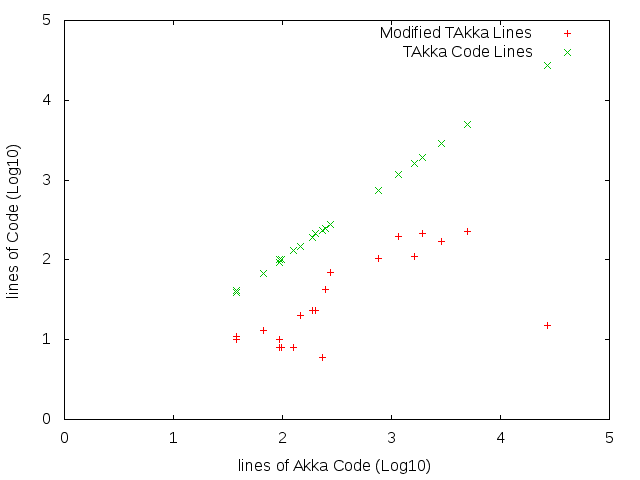
\includegraphics[scale=0.32]{Expressiveness/Expressiveness1.png}
        }
        \subfigure[Code Size: Relative Lines]{
           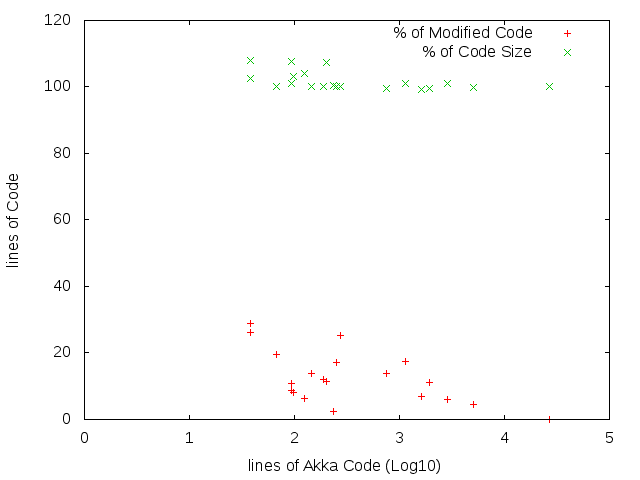
\includegraphics[scale=0.32]{Expressiveness/Expressiveness2.png}
        }
    \end{center}
    \caption{Code Size Evaluation}
   \label{fig:expressiveness}
\vspace{-10pt}   
\end{figure*}



\begin{figure*}[!ht]
     \begin{center}
        \subfigure[Throughput: Play]{
            \label{fig:play_throughput}
            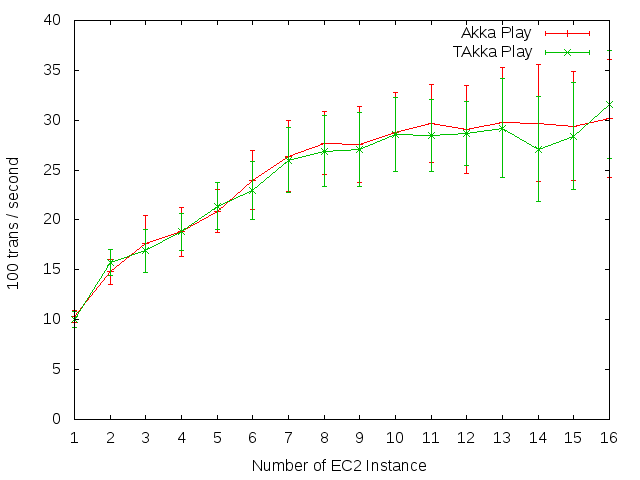
\includegraphics[scale=0.32]{TAkkaThroughput/Play_throughput.png}
        }
        \subfigure[Throughput: Socko]{
           \label{fig:socko_throughput}
           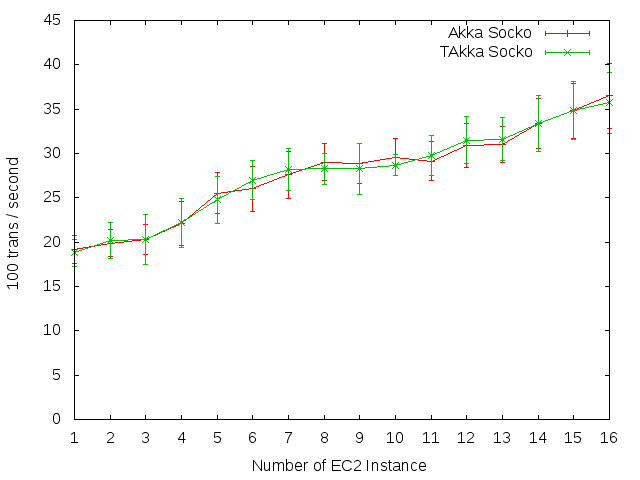
\includegraphics[scale=0.32]{TAkkaThroughput/Socko_throughput.png}
        }
    \end{center}
     \caption{Throughput Benchmarks}
   \label{throughput}
   \vspace{-10pt}
\end{figure*}

\begin{figure*}[!ht]
     \begin{center}
        \subfigure[Bang]{
            \label{fig:2_1}
            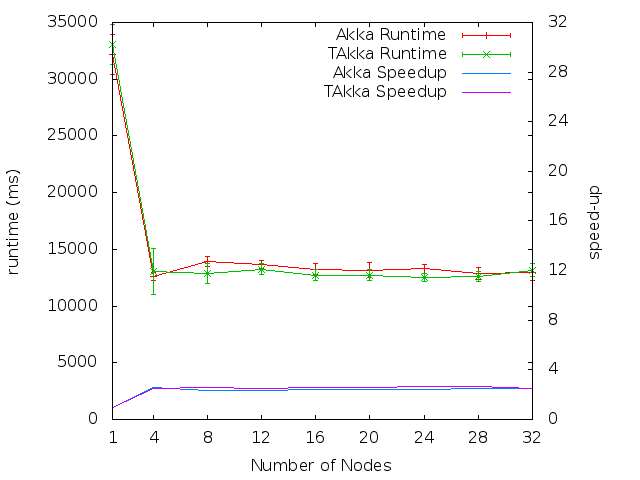
\includegraphics[scale=0.25]{efficiency/Bang.png}
        }
        \subfigure[Big]{
           \label{fig:2_2}
           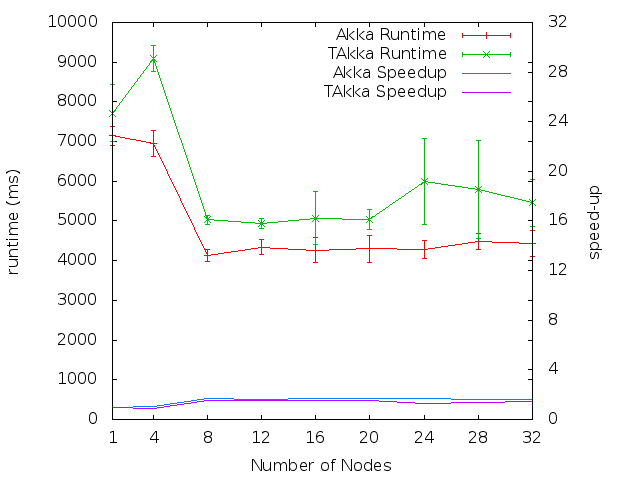
\includegraphics[scale=0.25]{efficiency/Big.png}
        }
        \subfigure[EHB]{
            \label{fig:2_3}
            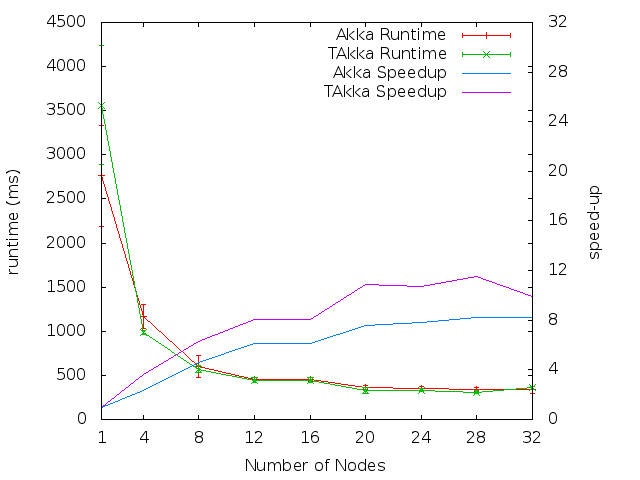
\includegraphics[scale=0.25]{efficiency/EHB.png}
        }\\
        \subfigure[MBrot]{
            \label{fig:2_5}
            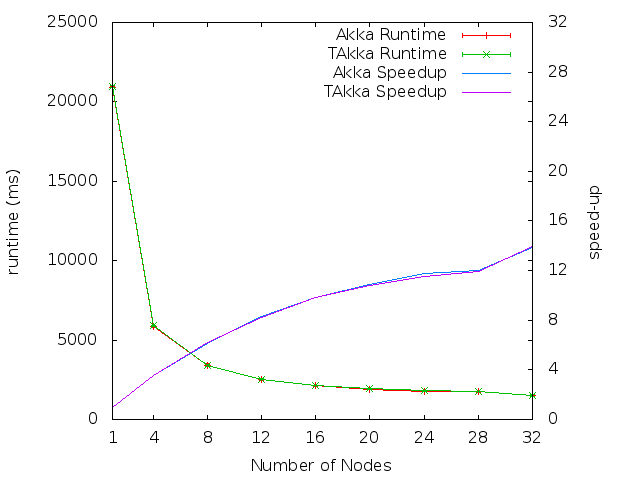
\includegraphics[scale=0.25]{efficiency/MBrot.png}
        }
        \subfigure[RAN]{
            \label{fig:2_7}
            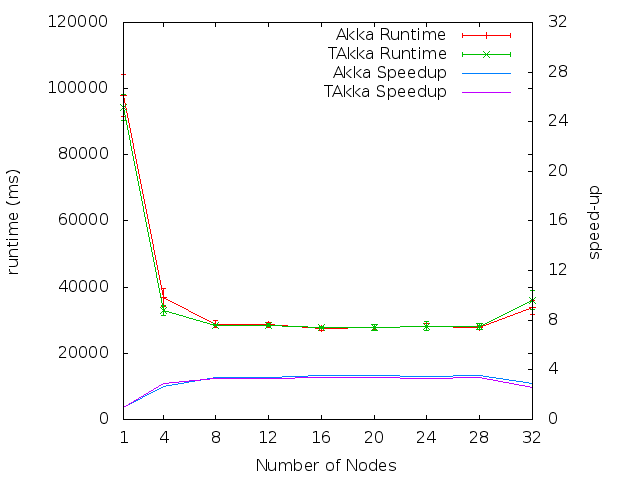
\includegraphics[scale=0.25]{efficiency/RAN.png}
        }
        \subfigure[SerialMsg]{
           \label{fig:2_8}
           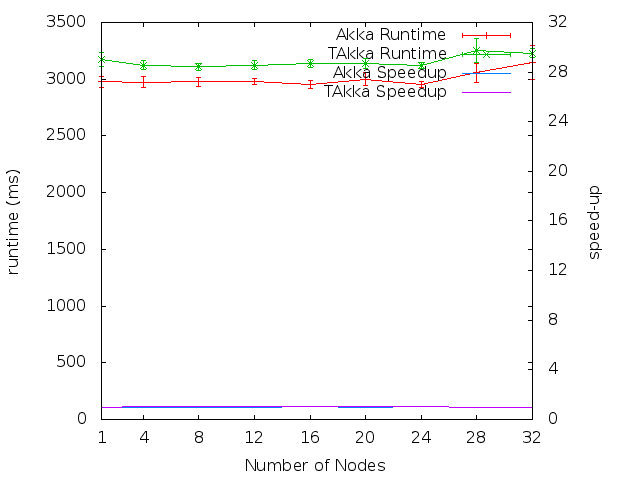
\includegraphics[scale=0.25]{efficiency/SerialMsg.png}
        }\\
    \end{center}
    \caption{Runtime \& Scalability Benchmarks}
   \label{runtime}
   \vspace{-10pt}
\end{figure*}

This section investigates whether the type discipline enforced by TAkka restricts the 
expressibility of Akka.  Table~\ref{express} lists the examples used for expressiveness checks.  
Examples are selected from Quviq \citep{quviq}
and open source Akka projects to ensure that the main requirements for actor 
programming are not unintentionally neglected.  Examples from 
Quviq are re-implemented using both Akka and TAkka.  Examples from 
Akka projects are re-implemented using TAkka.  Following standard practice,  
we assess the overall code modification and code 
size by calculating the geometric mean of all examples \citep{HePa06}. The evaluation results 
in Table~\ref{express} show that when porting an Akka program to TAkka, about 
8.5\% lines of code need to be modified including additional type declarations. 
Sometimes, the code size can be smaller because TAkka code does not 
need to handle unexpected messages.  On average, the total program size 
of Akka and TAkka applications are almost the same.  Figure~\ref{fig:expressiveness}
reports the same result in a Scatter chart.

A type error is reported by the compiler when porting the Socko example 
\citep{SOCKO} from its Akka implementation to its equivalent TAkka 
implementation. Socko is a library for building event-driven web services.  The 
Socko designer defines a {\tt SockoEvent} class to be the supertype of all 
events.  One subtype of {\tt SockoEvent} is {\tt HttpRequestEvent}, 
representing events generated when an HTTP request is received. The designer 
further implements subclasses of the {\tt Method} class, whose {\tt unapply} 
method is intended to have an output of type {\tt Option[HttpRequestEvent]}.  
The Socko designer made a type error in the method declaration so that the {\tt 
unapply} has output type {\tt Option[SockoEvent]}. The type error is not 
exposed in test examples because those examples only test HTTP events. 
The design flaw is exposed when rewriting Socko using TAkka.



% \vspace{-5pt}
\section{Throughput and Scalability}
\label{efficiency}
This section investigates whether managing type information in TAkka reduces
performance.  The TAkka library is built on Akka so that code for shared features 
can be re-used.  The three main sources of overheads in the TAkka implementation
are: (i) the cost of adding an additional operational layer on top of Akka 
code, (ii) the cost of constructing type descriptors, and (iii) the cost of 
transmitting type descriptors in distributed settings. We assess the effects of
the above overheads in terms of throughput and scalability.

The example used in the throughput benchmark is the JSON serialization example 
\citep{techempower}.  The example was implemented using Akka Play, TAkka Play, Akka 
Socko, and TAkka Socko.  All four versions of the web service are deployed to 
Amazon EC2 Micro instances (t1.micro), each of which has 0.615GB memory. The throughput 
is tested with up to 16 EC2 Micro instances.  For each number of EC2 instances, 
10 rounds of throughput measurement are executed to gather the average and 
standard deviation of the throughput. The results reported in Figure~\ref{throughput} show that web servers built using the Akka-based library and 
the TAkka-based library have very similar throughput.


We further investigate the speed-up of multi-node TAkka applications by 
porting 6  BenchErl benchmarks \citep{RELEASE} which do not involve Erlang/OTP 
specific features.  Each BenchErl benchmark spawns one master process and 
many child processes for a given task.  Each child process performs 
a certain amount of computation and reports the result to the master process.  
The benchmarks are run on a 32 node Beowulf cluster at Heriot-Watt 
University. Each Beowulf node comprises eight Intel 5506 cores running at
2.13GHz. All machines run under Linux CentOS 5.5. The Beowulf nodes are
connected with a Baystack 5510-48T switch.

Figures \ref{runtime} reports the results of the BenchErl 
benchmarks.   We report the average and the standard deviation 
of the run-time of each example.  Depending on the ratio of the computation 
time and the I/O time, benchmark examples scale at different levels.  In 
all examples, TAkka and Akka implementations have almost identical 
run-time and scalability.

In the BenchErl examples, child processes are asked to 
execute the same computation a number of times.  In contrast, distributed and 
cluster computing techniques are often used to solve a computationally 
expensive task by distributing sub-tasks to independent nodes.  To simulate 
such a scenario, another benchmark, N-Queens Puzzle \citep{wiki:nqueens}, is added. 
Finding all solutions of an N-Queen Puzzle is an NP-hard problem.  Therefore, a 
suitable $n$ makes the problem a good benchmark to demonstrate the advantage of 
cluster and distributed programming.  Figure~\ref{nqueens_efficiency}
reports the result when $n$ is set to $14$.  The result shows that both the Akka and 
TAkka implementation have good scalability and similar efficiency.


\begin{figure}[!h]
     \begin{center}
        \subfigure[N-Queens Time]{
            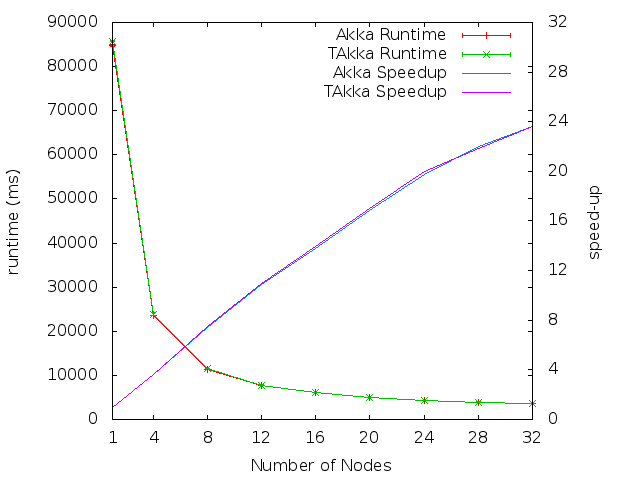
\includegraphics[scale=0.26]{efficiency/NQueens.png}
        }
    \end{center}
    \caption{Benchmark: N-Queens Puzzle}
   \label{nqueens_efficiency}
   \vspace{-10pt}
\end{figure}


\section{Conclusion}
\label{conclusion}

The Akka library accepts dynamically typed messages.  The TAkka
library introduces a type-parameter for actor-related classes. The additional 
type-parameter specifies the communication interface of 
that actor.  With the help of type-parameterized actors, unexpected 
messages to actors are rejected at compile time.
% In addition to eliminating programming bugs and type errors, 
% programmers would like to have a failure recovery mechanism for
% unexpected run-time errors.  
We have shown that type-parameterized 
actors can form supervision trees in the same way as untyped actors (Section~\ref{takka_design}).
We have shown that
adding type parameter does not restrict expressiveness, and requires
only small amounts of refactoring (Section~\ref{expressiveness}).  We have
shown that TAkka does not introduced performance penalties (Section~\ref{efficiency}), 
with respect to throughput, efficiency, and scalability.  The above results are encouraging for the 
use of types and supervision trees to implement reliable applications and improve the 
reliability of legacy applications with little effort.  
% We expect similar 
% results can be obtained in other actor libraries.



\section{Acknowledgements}

The authors gratefully acknowledge the substantial help they have received from 
many colleagues who have shared their related results and ideas with us over 
the long period during which this paper was in preparation.  
Benedict Kavanagh and Danel Ahman for continuous comments and discussions.
The RELEASE team for giving us access to the source code of the BenchErl 
benchmark examples.  Thomas Arts from Quviq.com and Francesco Cesarini from 
Erlang Solutions for providing the Erlang source code of two examples used in their 
commercial training courses.


\bibliographystyle{abbrv}
\bibliography{takka}  % sigproc.bib is the name of the Bibliography in this case
% You must have a proper ".bib" file
%  and remember to run:
% latex bibtex latex latex
% to resolve all references
%
% ACM needs 'a single self-contained file'!
%


\end{document}
